\section{Treasury System Overview\label{sec:overview}}

The decentralized nature of blockchain systems complicates their maintenance, further development and governance. System improvements have to be publicly proposed, approved, and funded, keeping the corresponding level of decentralization. 

To that end, it is important to provide a sustainable decentralized treasury system, which is oriented towards governing funds for recurring tasks of the blockchain development, maintenance and support. Having this component is important for maintaining a decentralized system in the long-term prospective.

The basis of the treasury system is a collaborative decision-making process which can be done through the voting. A key feature expected from the voting procedure is the absence of a centralized control over the operational process. That is, it must neither rely on trusted parties or powerfull minority, nor introduce incentives to their appearance. Ideally, all cryptocurrency stake holders are entitled to participate in the decision-making process. 

The basic flow of a decision making process is depicted in Fig.\ref{fig:DMP}. In the first stage a proposal is submitted for consideration to the community (e.g. provide xxx coins from the treasury for a specific  development team to implement feature Y). The second stage is voting where corresponding participants of the system express their opinion by posting voting ballots on a blockchain. To achieve better collaborative intelligence, it is allowed to delegate the voting power to a special actor called \textit{expert}. In the third stage the system processes ballots, counts votes and concludes a decision. In the final stage the decision is executed (e.g. the coins are transferred from treasury to the development team).

\begin{figure}[htbp]
	\centering
	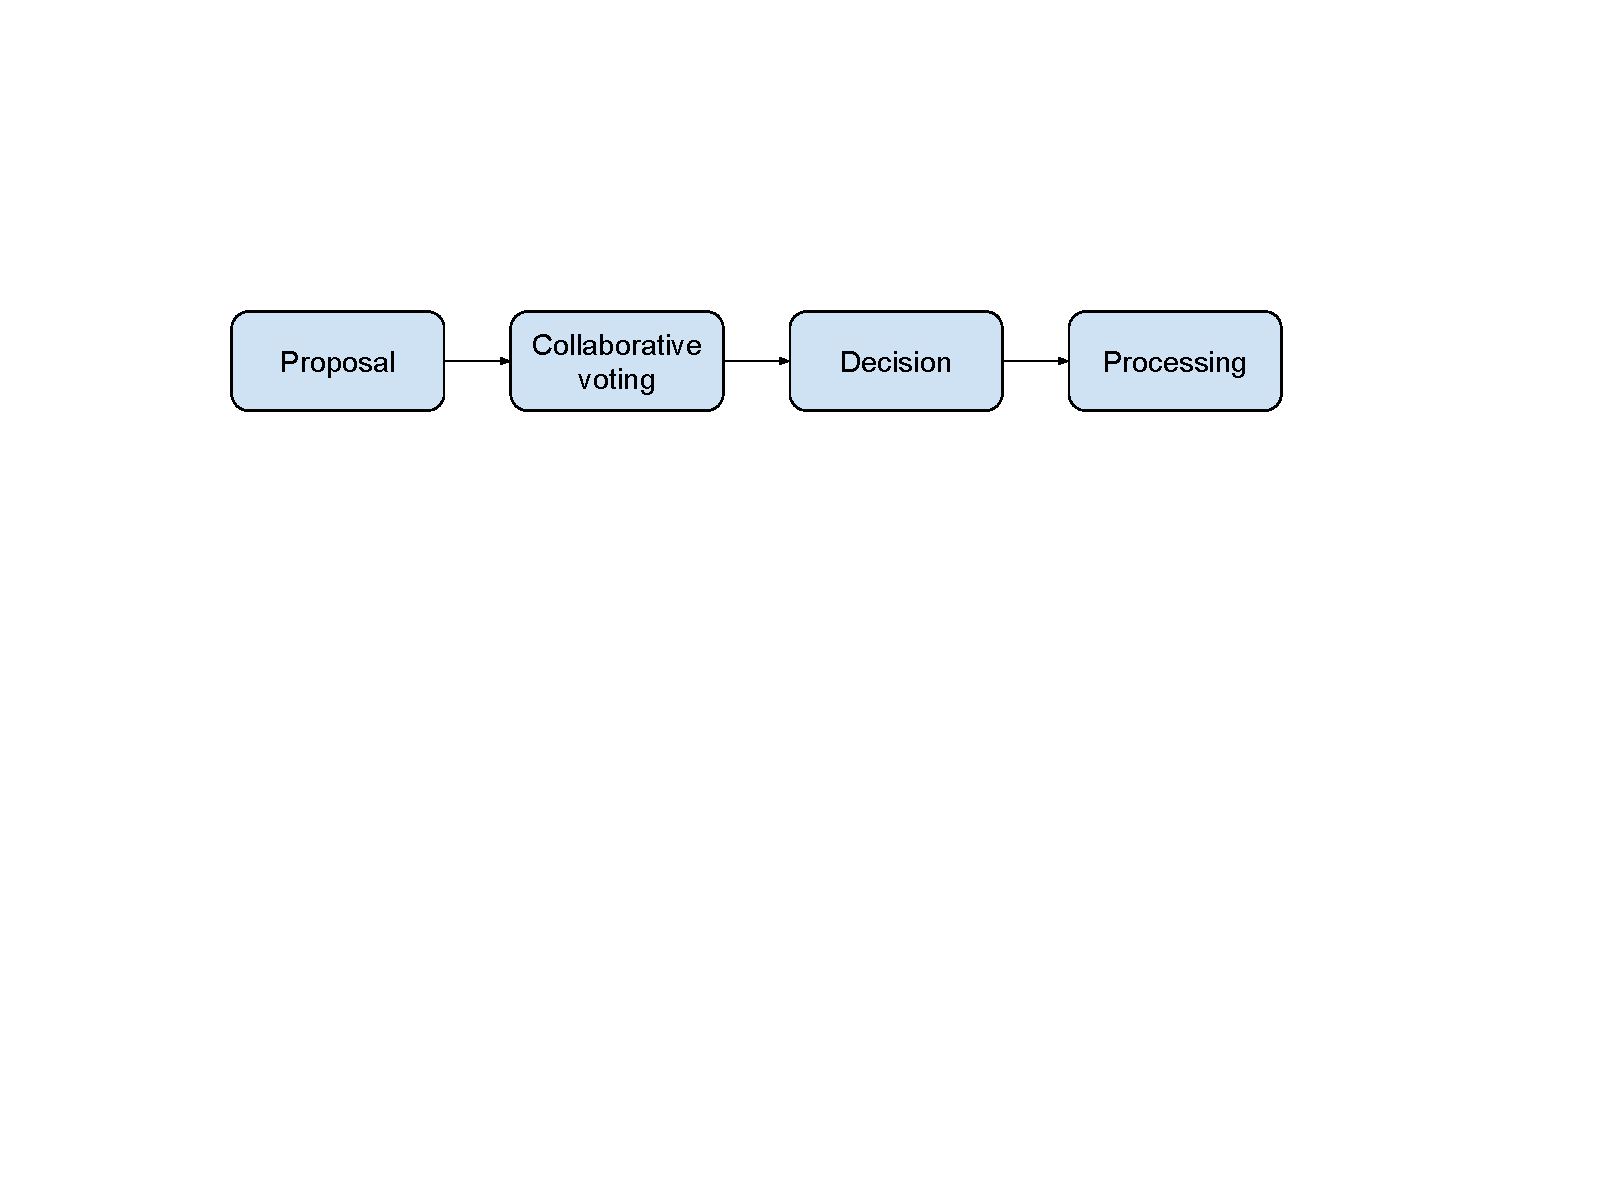
\includegraphics[trim={3cm 13cm 4cm 5cm}, clip,width=1\columnwidth] {DMP.pdf}
	\caption{Basic flow of a decision-making process}
	\label{fig:DMP}
\end{figure}

This process is repeated periodically. Each such period is called a treasury epoch. In our treasury system, each epoch consists of the following stages:
\begin{enumerate}[leftmargin=5em, itemsep=0em]
    \item \textbf{Pre-voting stage}.
        \subitem a) Proposals submission.
        \subitem b) Voters/Experts/Committee registration.
        \subitem c) Randomness revealing.
        \subitem d) Randomized selection of the voting comittee.
        \subitem a) Distributed voting key generation.
    \item \textbf{Voting stage}.
        \subitem a) Ballots casting.
    \item \textbf{Post-voting stage}.
        \subitem a) Joint decryption of tally.
        \subitem b) Randomness commitment for the next epoch.
        \subitem c) Execution.
\end{enumerate}

\subsection{Pre-voting Stage}
\textbf{Entities}. All stake holders are eligible to participate in case they registered themselves. The stake holders may have one or more of the following roles.
\begin{itemize}[leftmargin=5em, itemsep=0em]
    \item \textbf{Project owners} $\mathcal{O}:=\{o_1,\ldots, o_k \}$, who submit proposals for funding;
    \item \textbf{Voting committee} $\mathcal{C}:=\{c_1,\ldots, c_l \}$ - special actors that maintain a decentrilized voting procedure (e.g., generate a shared voting public key and collectively decrypt the voting result);
    \item \textbf{Voters} $\mathcal{V}:=\{v_1,\ldots, v_n \}$ - a set of stake holders that deposited a certain amount of stake to participate in voting; the voting power is proportional to the amount of deposited stake;
    \item \textbf{Experts} $\mathcal{E}:=\{e_1,\ldots, e_m \}$ - a special type of voters that have specialist knowledge and expertise in some field; their voting power equals to the sum of voting power of all regular voters that delegated their stake to the expert.
\end{itemize}
Note that experts and voting committee members are also required to deposit some fixed amount of stake to register themselves. But this stake does not provide them voting power, but rather serves as a deterrence against malicious behaviour. In case they do not follow the protocol, the deposit is confiscated.
	
The deposited stake of all entities is locked for a certain amount of time (e.g., several epochs) to incentivize prudent behaviour.
\\~\\
\textbf{Proposal submission}. In order to submit a proposal for funding, a project owner submits a special proposal transaction\footnote{See the implementation of a proposal transaction here:\\ \href{https://github.com/input-output-hk/TreasuryCoin/blob/master/examples/src/main/scala/examples/hybrid/transaction/ProposalTransaction.scala}{https://github.com/input-output-hk/TreasuryCoin/.../examples/hybrid/transaction/ProposalTransaction.scala}} to the blockchain:
\[Proposal_{TX}\ \stackrel{\mathrm{def}}{=}\ (projectID,\ recipientAddr,\ amount),\]
where:
\begin{conditions}
    projectID & a unique identifier of the project (e.g., its name); \\
    recipientAddr &  address of the recipient, where requested funds should be sent in case of approval; \\
    amount &  requested amount of funds.
\end{conditions}

Note that to prevent denial-of-service attacks it is required for the submitter to burn some amount of coins.
\\~\\
\textbf{Voters/Experts registration}. In order to become a voter or expert, a stakeholder must submit the following registration transaction\footnote{See the implementation of a registration transaction here:\\ \href{https://github.com/input-output-hk/TreasuryCoin/blob/master/examples/src/main/scala/examples/hybrid/transaction/RegisterTransaction.scala}{https://github.com/input-output-hk/TreasuryCoin/.../examples/hybrid/transaction/RegisterTransaction.scala}}:
\label{ref:reg_tx}
\[Reg_{TX}\ \stackrel{\mathrm{def}}{=}\ (role,\ Option[committeePubKey],\ pubKey,\ depositAmount,\ paybackAddress,\ sig),\]
where:
\begin{conditions}
    role & a role for which a stakeholder is registered (voter or expert); \\
    committeePubKey &  an optional field; in case a voter/expert also wants to participate in the voting committee, he provides an additional public key that is used for committee-specific operations; \\
    depositAmount &  an amount of stake that a voter wants to deposit to acquire the right to participate in the voting process; the voting power is proportional to the amount of deposited stake. In case a voter also wants to be a committee member, he deposits an additional fixed amount of stake, which does not increase his voting power. In case registering an expert, deposited stake is a fixed amount only depending on if the expert also wants to participate in the committee. Experts do not have their own voting power; \\
    paybackAddress & an address where rewards should be sent; \\
    pubKey & a personal public key that will be used for issuing ballots; \\
    sig & a signature on the whole registration transaction issued with \textit{pubKey}.
\end{conditions}

\textbf{Randomness revealing.} A random value is required for the committee selection procedure. This random value is generated collectively by the voting committee of the previous treasury epoch. At this stage, they just reveal previously committed randomness. It is crucial that the randomness is revealed after the registration phase, so that committee candidates cannot influence the selection procedure by adjusting their registration data.

\textbf{Randomized selection of the voting comittee.} To facilitate efficiency of the voting protocol, a voting committee is restricted to have fixed size. Since there might be more users wanting to participate in the committee, a special random selection procedure (Fig.~\ref{committee_select}) is used to determine who will be in the committee for a particular treasury epoch\footnote{See implementation here:\\ \href{https://github.com/input-output-hk/TreasuryCoin/blob/master/examples/src/main/scala/examples/hybrid/state/TreasuryState.scala\#L367}{https://github.com/input-output-hk/TreasuryCoin/../examples/hybrid/state/TreasuryState.scala:selectApprovedCommittee()}}.

% \begin{protocolframe}{\textbf{Committee Selection Procedure}}
\myhalfbox{Committee Selection Procedure}{white!40}{white!10}{
\begin{enumerate}
    \item For each committee member $C_i$ calculate the value
    \[t_i=H(committeePubKey_i\ |\ randomness),\]
    where $randomness$ is some random value derived after the registration procedure has been finished (e.g., it can be a randomness derived from a blockchain or collectively generated by committee members of the previous epoch).
    \item Sort all registered committee members by their $t_i$ values.
    \item Chose top $l$ committee members, where $l$ is a system parameter, who constitute the voting committee for the current treasury epoch. 
\end{enumerate}
% \end{protocolframe}
}{Committee Selection Procedure\label{committee_select}}

\textbf{Distributed key generation}. During the DKG phase, the elected voting committee jointly generates a shared public voting key which will be used by voters and experts to encrypt their ballots. Then, after the voting stage is finished, the committee collectively decrypt the tally and generate randomness for the next treasury epoch.

\subsection{Voting Stage}
After the preparation stage there are a set of proposals $\mathcal{P}:=\{P_1,\ldots, P_k \}$ and three sets of voting participants:
\begin{enumerate}
    \item \textbf{Voters} $\mathcal{V}:=\{v_1,\ldots, v_n \}$. Each voter is associated with his registered $pubKey_{v_i}$ and voting power $vp_{v_i}$.
    \item \textbf{Experts} $\mathcal{E}:=\{e_1,\ldots, e_m \}$. Each expert is associated with his registered $pubKey_{e_i}$ and his number $i$. 
    \item \textbf{Committee members} $\mathcal{C}:=\{c_1,\ldots, c_l \}$. Each committee member is associated with two registered keys $pubKey_{c_i}$ and $committeePubKey_{c_i}$. The latter is used to encrypt communication with other committee members.
\end{enumerate}

During the voting stage, voters and experts issue voting ballots where they put their choices regarding proposals. For each proposal, a voter may chose among three options: Yes, No, Abstain, or he can delegate his voting power to some expert, in which case the chose of the expert will be counted with the corresponding voting power of the voter.
Note that each proposal is treated separately, so that a voter can delegate his voting power to different experts for different proposals.

\subsection{Post-voting Stage}

\textbf{Joint decryption of tally}. After the voting stage, all ballots are collected and the voting committee jointly decrypt the tally for each proposal without revealing personal choices of voters and experts. Winning proposals are selected according to the procedure on Fig.~\ref{fig:proposals_select}.

\myhalfbox{Proposals selection procedure}{white!40}{white!10}{
\begin{enumerate}
    \item Filter out all proposals for which the difference between "Yes" and "No" votes is less than 10\% of the total voting power.
    \item Sort all remaining proposals according to the amount of "Yes" votes (taking into account the voting power of different voters).
    \item Top ranked proposals are funded one-by-one until the treasury budget for the epoch is exhausted. 
\end{enumerate}
}{Proposals selection procedure\label{fig:proposals_select}}

\newpage
\textbf{Randomness commitment for the next epoch}. At this stage, each committee member commits a random value that will be used to construct randomness for the next treasury epoch.

\textbf{Execution}. During the execution stage treasury funds are distributed to winning proposals. Certain proportion (e.g. 20\%) of the treasury fund is used to reward the voting committee members, voters and experts.

\subsection{Incentives}

There are three main factors to incentivize treasury participants:
\begin{enumerate}
	\item Rewards.
	\item Deposit lock.
	\item Deposit confiscation.
\end{enumerate}

\textbf{Rewards}. The cornestone of the incentive scheme is the rewards paid for participating in the treasury protocol. All entities are eligible for rewards according to their roles. The rewards fund is a fixed portion (e.g., 20\%) of the overall treasury fund, which is divided between committe members and voters. Voting committee members receive a fixed amount of reward, while voters receive rewards proportional to their voting power. Experts receive rewards as a percentage (e.g. 5\%) of rewards for voters, who delegated to them\footnote{See implementation of payments distribution here:\\ \href{https://github.com/input-output-hk/TreasuryCoin/blob/master/examples/src/main/scala/examples/hybrid/state/TreasuryState.scala\#L537}{https://github.com/input-output-hk/TreasuryCoin/../examples/hybrid/state/TreasuryState.scala:getPayments()}}.

The rewards are paid only if an entity follows the protocol correctly. For voters and experts it means that they issue correctly formed voting ballots in time; for committee members it means that they follow the protocol and issue all required transactions in time.

\textbf{Deposit lock}. All entities are required to deposit certain amount of stake depending on their roles. This deposit is locked for a prolonged period of time (e.g., 3 treasury epochs). The basic idea behind it is to establish an incentive for voters to make sensible decisions that will benefit long-term prospects of the system. Given that their stake is locked they are incentivized to make decisions that will increase value of their stake.

\textbf{Deposit confiscation}. Deposit confiscation is applied to experts and committee members in case they do not behave as expected. Given that experts are responsible to make decisions for voters delegating to them, their refusal to participate in a voting (i.e., not issuing a ballot) is considered as malicious behaviour that is punished by deposit confiscation.

Committee members are responsible for managing the voting procedure. Even though the protocol is robust against failure of up to 50\% of members, a committee member is punished by deposit confiscation in case of not following the protocol.